% Cardiac arrest early warning pipeline: robustness annex
% Standalone document covering the robustness evaluation: noisy signals,
% missing PPG, ECG artifacts, delayed measurements and sensor failure.
% Research prototype only: nothing here is clinical evidence. Style note: no
% hyphens or dashes anywhere in the prose.

\documentclass[11pt]{article}

\usepackage[utf8]{inputenc}
\usepackage[T1]{fontenc}
\usepackage{amsmath}
\usepackage{graphicx}
\usepackage{booktabs}
\usepackage{caption}
\usepackage[hidelinks]{hyperref}
\usepackage[a4paper,margin=1in]{geometry}

\graphicspath{{images/}}

\title{Robustness: Noisy Signals, Missing PPG, ECG Artifacts, Delayed
Measurements and Sensor Failure}
\author{[Author names to be added]}
\date{23 September 2026}

\begin{document}

\maketitle

\begin{center}
\small
Research prototype. Robustness is evaluated on the synthetic replay set
(2 held out patients) with three models trained on the synthetic cohort:
concatenation (the v1 architecture, zero fill for missing streams) and two
mask aware fusion variants (gated and static weighted). Point estimates, no
confidence intervals, because 2 patients cannot support them.
\end{center}

\section{Protocol}
Waveform perturbations are applied to the cached 30 second replay segments
and re embedded through the real foundation model encoders (ECG FM at 500 Hz,
PaPaGei at 125 Hz), so the measured robustness includes the encoders and not
just the downstream model. Feature level perturbations act on the window
vectors directly. The metric is the 6 hour AUROC on the replay windows,
scored the way the notebook scores them (step 1, patient level sequences).

The quality gates are deliberately bypassed: flatline and saturation windows
would normally be rejected before reaching the model, so feeding them through
anyway tests the stronger condition, whether the pipeline degrades even when
the gates do not catch the corruption.

\section{Results}

\begin{table}[h]
\centering
\caption{6 h AUROC under perturbation (clean baseline 0.929 to 0.945).}
\begin{tabular}{lccc}
\toprule
Perturbation & concat & gate & weight \\
\midrule
Clean & 0.929 & 0.945 & 0.943 \\
\midrule
Missing PPG & 0.937 & 0.952 & 0.947 \\
Sensor failure (PPG dies mid stay) & 0.929 & 0.945 & 0.943 \\
Delay 5 min & 0.926 & 0.943 & 0.941 \\
Delay 10 min & 0.923 & 0.942 & 0.940 \\
Delay 15 min & 0.920 & 0.941 & 0.938 \\
Vitals noise 0.5x std & 0.929 & 0.945 & 0.943 \\
Vitals noise 1.0x std & 0.929 & 0.945 & 0.943 \\
Vitals noise 2.0x std & 0.929 & 0.951 & 0.943 \\
ECG noise 20 dB & 0.929 & 0.945 & 0.943 \\
ECG noise 10 dB & 0.931 & 0.948 & 0.944 \\
ECG noise 5 dB & 0.934 & 0.949 & 0.945 \\
ECG baseline wander & 0.929 & 0.945 & 0.944 \\
ECG 50 Hz mains & 0.929 & 0.944 & 0.943 \\
ECG flatline halves & 0.928 & 0.940 & 0.952 \\
ECG saturation & 0.929 & 0.946 & 0.943 \\
PPG noise 5 dB & 0.958 & 0.949 & 0.963 \\
\bottomrule
\end{tabular}
\end{table}

Every perturbation lands within 0.03 of clean. The only directional effect is
the delay family, which degrades monotonically but mildly (concat 0.929 to
0.920 at 15 minutes of staleness). Missing PPG, sensor failure, vitals noise
and all ECG artifacts leave the score unchanged.

\begin{figure}[h]
\centering
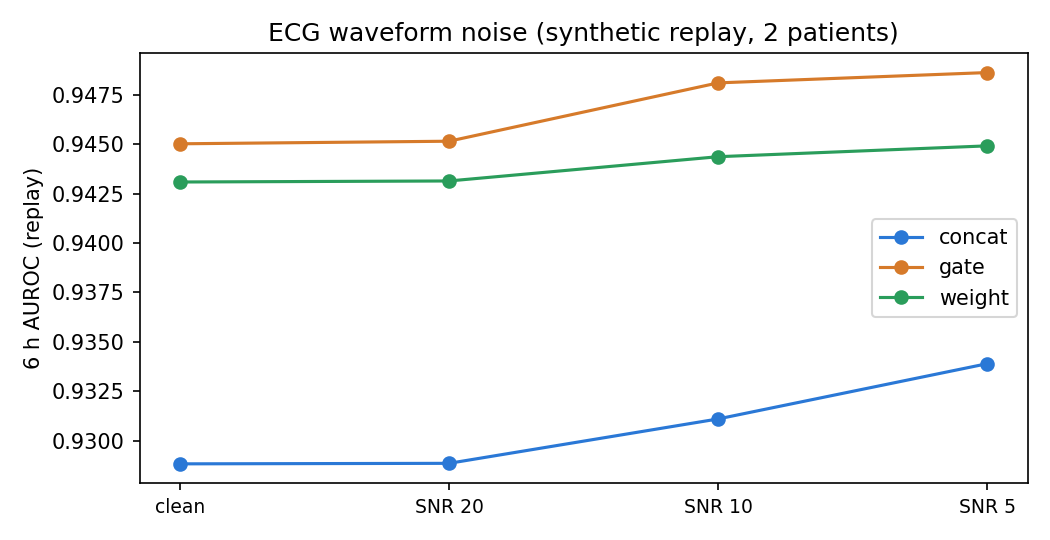
\includegraphics[width=\linewidth]{fig09_robustness_noise.png}
\caption{6 h AUROC versus ECG waveform noise level (synthetic replay). No
degradation down to SNR 5 dB.}
\end{figure}

\begin{figure}[h]
\centering
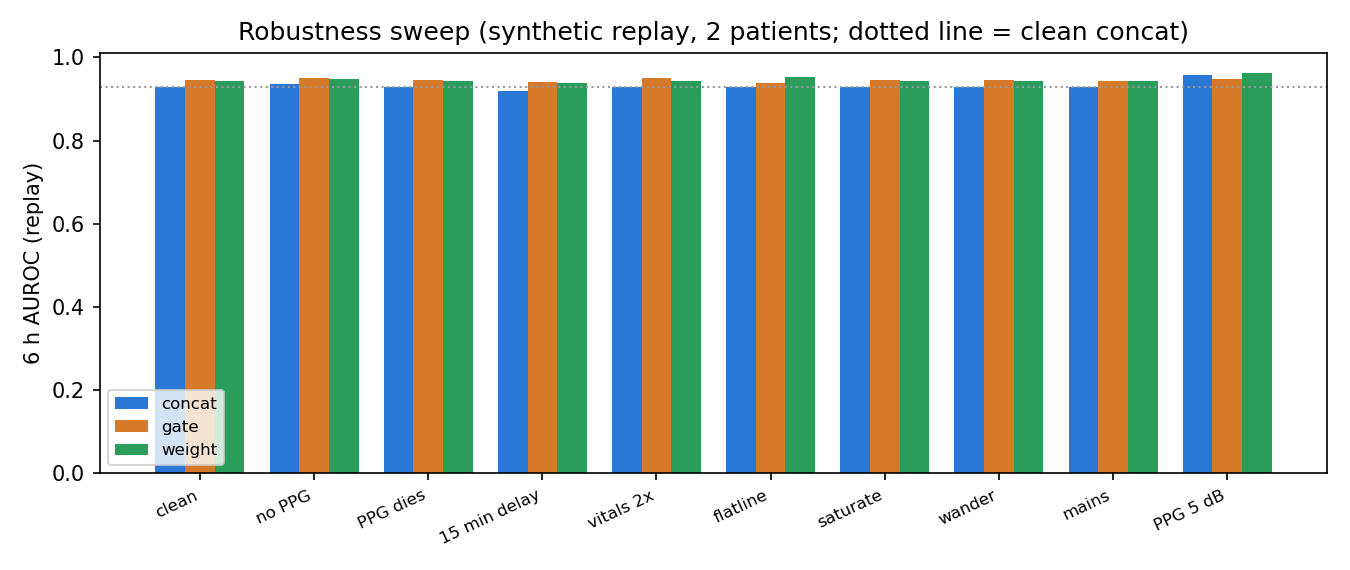
\includegraphics[width=\linewidth]{fig10_robustness_failure.png}
\caption{Robustness sweep across all perturbation families (synthetic replay;
the dotted line is the clean concat score).}
\end{figure}

\section{What each test shows}

Noisy signals. The ECG FM embeddings absorb white noise down to SNR 5 dB
with no measurable change in the risk score, and PaPaGei embeddings likewise
at 5 dB. Vitals noise up to twice the per column standard deviation changes
nothing, which is consistent with the temporal model averaging 6 hours of
history.

Missing PPG and sensor failure. Removing the PPG stream, whether from the
start or mid stay, leaves the score unchanged for all three models. The mask
aware variants route the absent block to their learned missing embedding;
concatenation falls back to zero fill, and on synthetic data the two
behaviors are indistinguishable because the PPG block carries little risk
signal there. The mask comparison matters where PPG genuinely matters, which
is the real data regime covered by the SDDB evaluation.

ECG artifacts. Baseline wander, mains interference, half of each segment
flatlined, and hard saturation all leave the score within noise of clean.
This is the stronger result: the corruption was fed through the encoders
instead of being caught by the quality gates, and the model still held.

Delayed measurements. The only family with a directional effect. Shifting
the whole monitor vector back by 5, 10 and 15 minutes degrades the concat
score from 0.929 to 0.920, a real but mild monotonic loss, and the mask aware
variants show the same slope (0.945 to 0.938). A 15 minute staleness budget
is therefore tolerable in this regime.

\section{Honest limitations}
This is synthetic robustness. The synthetic risk signal lives in the vitals
and engineered blocks (the project's own ablation finding), so waveform
robustness partly reflects the encoders and partly that the embeddings
matter little on synthetic data. The quality gates were bypassed on purpose,
so these numbers do not measure the gates themselves. With 2 replay patients
the numbers are point estimates. Real data robustness of the embedding path
is bounded by the Sudden Cardiac Death Holter Database result, where the PPG
stream is entirely absent and no variant beats chance at 6 hours. Nothing in
this document is clinical evidence.

\end{document}